\chapter{Construction of Occurrence Graph Grammars}\label{ch:tests}

%A test case is a collection of (1) input values necessary to complete some execution of the system under testing, (2) the results that must be produced after executing the test (assuming the system satisfies the intended behaviour) and (3) any inputs necessary to setup the system into the appropriate state to receive the test values~\cite{Ammann2008}.
%Test oracles are specifications describing properties about the validity of tests cases, i.e. if the test must fail or pass. These properties may include relationships between the input given and the expected output, data validity properties, format of possible execution paths, etc. No matter the oracle format, it must be able to determine the validity of tests in a finite and reasonable amount of time~\cite{Weyuker1982}.

%In the following, we show how to use \newadd{deterministic} occurrence graph grammars to generate test cases and oracles from (simply-typed) graph grammars modelling systems. In theory, this approach can be used to generate tests for any graph grammar\footnote{\newadd{Assuming the grammar follows the DPO approach with incremental NACs}}, since it is based only on the properties of the formalism. However, we focused on graph grammars that were generated from use cases by using the methodology presented in \cite{Junior2015}, \cite{BezerraWEIT2016} and \cite{Cota2017}.

%This methodology is a systematic, computer-aided way to extract graph grammars from use cases or other text-based requirement documents. At the same time, it helps finding problems such as ambiguities, inconsistencies and omissions in the documents. Thus, providing a better specification and also an improved model. By generating tests from these grammars we are indirectly generating tests for the underlying use cases. The test generation, to be described in next sections, was implemented in Verigraph as an extension of the previously discussed calculation of occurrence graph grammars.

%We focused our approach on testing the integration of different functionalities (or requirements) of a system. By \emph{functionality}, we informally mean an aim the system is supposed to accomplish, which has value to a user or any other stakeholder. By \emph{integration} we mean the emergent behaviour of executing several functionalities, possibly multiple times.

% In the graph grammar model of a system, a functionality can be represented either as a single rule or as a collection of rules. In either case, those rules must be executed to achieve the functionality goals. Therefore, the main idea of our approach is that, given a collection of functionalities, we find out whether it is possible to find a sequence in which all these functionalities can be performed, then we characterize the assumptions that must be satisfied for them to be performed and/or the restrictions that may prevent their execution. Given a collection of functionalities modelled as graph rules, we are interested in generating:

\iffalse
\begin{enumerate}
\item the minimal input data necessary for these functionalities to execute, as well as the output data of a successful execution;
\item at least one path in which all functionalities can be applied (if possible);
\item a set of constraints two characterize any test into those which should pass and those which should fail;

\hide{
\item a set of constraints which can tell which intermediate states of the system are valid and those that are not.}
\end{enumerate}

Notice that the two first items correspond to test cases while the last one correspond to test oracles.
\fi
%First, we present a brief overview of the methodology for extracting graph grammars from use cases, after what we present the process of generating the tests cases from the extracted grammars.

\section{Running Example: A Restaurant System}

We begin by presenting a running example: a graph grammar that models a a restaurant system. This grammar was built from the set of use cases presented in Appendix~\ref{app:use-cases} by applying the systematic methodology proposed by~\cite{Junior2015}. These use cases model basic functionalities of a restaurant system such as login of employees, reservation and cancellation of tables, accommodation of clients, serving tables, among others. While only some excerpts of this grammar are shown in this work, the complete extracted grammar can be found on appendix~\ref{app:use-cases} and at the Verites repository for case studies\footnote{https://github.com/Verites/case-studies}.

%Given the graph grammar model of a system, we want to generate test cases and oracles for collections of its underlying functionalities. These collections could represent something as ``atomic'' as a successful or failing login attempt or something as complex as the entire workflow of attending clients, which would require attendants and waiters to log in into the system, tables to be occupied, orders to be prepared, among possibly several other steps.

%The reason why we focused on collections of functionalities is to test the emergent behaviour of a system, which usually is not observable if we consider each functionality in isolation. By grouping together several (usually, but not necessarily different) functionalities, we may realize how they interact with each other and which are the overall effects of this integration.

%\begin{definition}[Functionality Collection] Given a graph grammar \graphGrammar{} that models a system, a \emph{functionality collection} $F$ is a collection of its grammar rules. The term collection here is used instead of set to imply that the same rule $r \in P$ can appear more than once in $F$. In this context, it means the functionality modelled by $r$ is intended to be executed more than once.
%\end{definition}

\begin{example} Figure~\ref{fig:tests:grammar} shows some of the rules which compose our grammar. The chosen rules represent one way in which the entire process of serving a client can be accomplished. In this particular case, we chose the rules representing the successful paths of the use cases \emph{reserve table}, \emph{accommodate client}, \emph{serve table} and \emph{close table}.

\begin{description}
  \item[Reserve table:] The receptionist of tags a table as reserved for a specific client at a given date and time, such that the reserved table can not be allocated for another client, either by accommodation or reservation, at the same time.
  \item[Accomodate client:] The receptionist lead the client to his/her previously reserved table, then notifies a waiter that this table is waiting for service.
  \item[Serve table:] The waiter goes to a table with clients to take the order, which consists of adding or removing items to the order, then closing it and sending it to the kitchen to be prepared.
  \item[Close table:] The waiter goes to a table that has been serviced, closes the bill and collects the payment from the client.
\end{description}

\begin{figure}[!ht]
  \centering
  \begin{subfigure}[t]{.5\textwidth}
    \centerline{\fbox{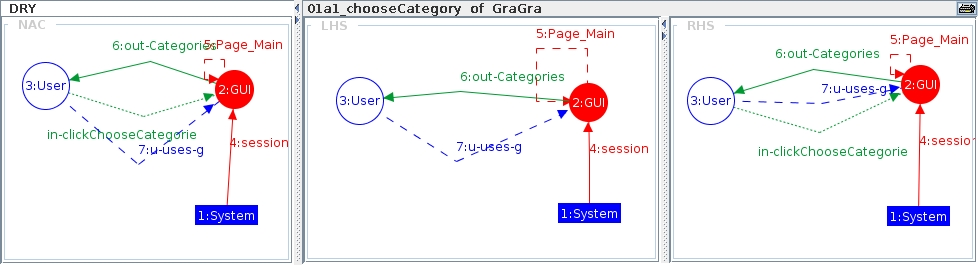
\includegraphics[scale=0.5]{images/generating-tests/grammar/rule01}}}
    \caption{Rule \emph{choose category}}
  \end{subfigure}
  \begin{subfigure}[t]{.5\textwidth}
    \centerline{\fbox{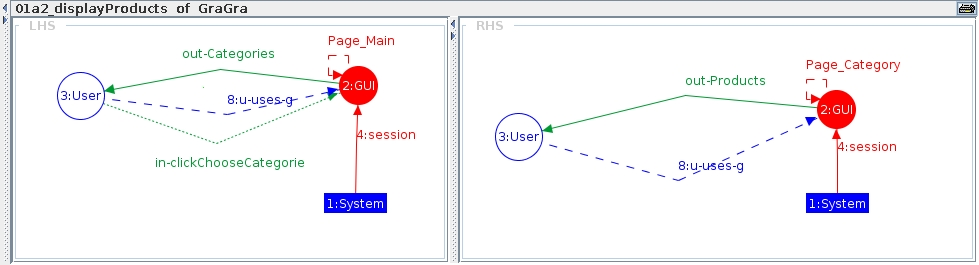
\includegraphics[scale=0.5]{images/generating-tests/grammar/rule02}}}
    \caption{Rule \emph{display products}}
  \end{subfigure}
  \begin{subfigure}[t]{.5\textwidth}
    \centerline{\fbox{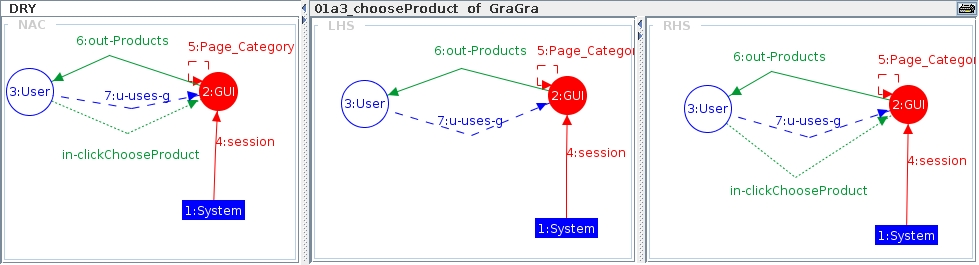
\includegraphics[scale=0.5]{images/generating-tests/grammar/rule03}}}
    \caption{Rule \emph{choose products}}
  \end{subfigure}
  \begin{subfigure}[t]{.5\textwidth}
    \centerline{\fbox{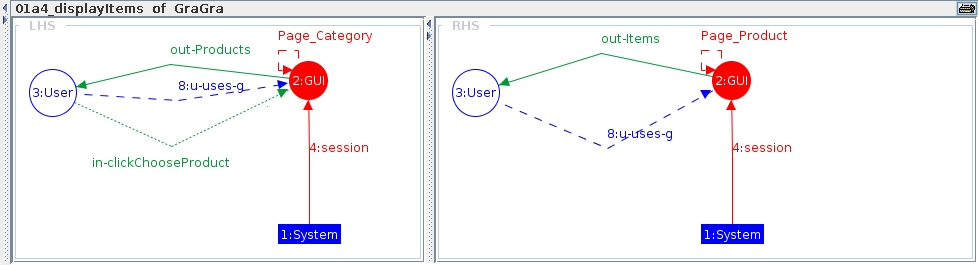
\includegraphics[scale=0.5]{images/generating-tests/grammar/rule04}}}
    \caption{Rule \emph{display items}}
  \end{subfigure}
  \caption{Rules for the use case \emph{browse catalogue}}\label{fig:tests:grammar}
\end{figure}

\begin{figure}[!]
\ContinuedFloat
\centering
  \begin{subfigure}[t]{.5\textwidth}
    \centerline{\fbox{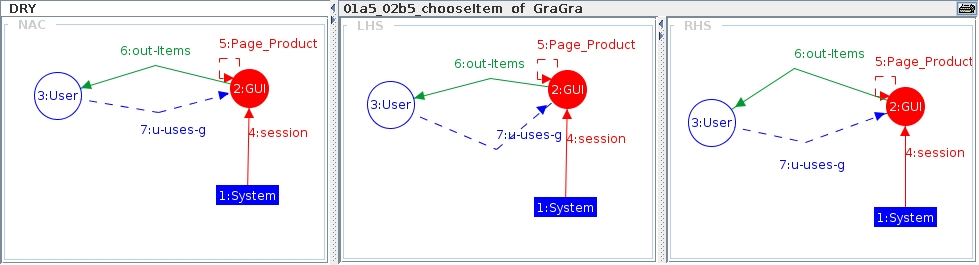
\includegraphics[scale=0.5]{images/generating-tests/grammar/rule05}}}
    \caption{Rule \emph{choose item}}
  \end{subfigure}

  \begin{subfigure}[t]{.5\textwidth}
    \centerline{\fbox{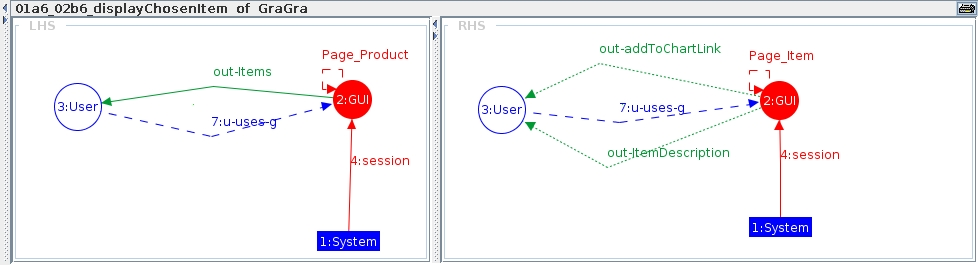
\includegraphics[scale=0.5]{images/generating-tests/grammar/rule06}}}
    \caption{Rule \emph{display chosen item}}
  \end{subfigure}
\end{figure}
\end{example}


\section{Preparing the input}

Along with the grammar $GG$ and a collection of rules $F$ based on $P$, we will also need a way of specifying how the rules will interact among themselves\footnote{ We use the term collection instead of set because, in this case, a rule can appear more than once and we need them to be accounted as such.}. Specifically, which elements (nodes and edges) are common throughout them. For this purpose, we create an \emph{input-output relation}, depicting connections between the rules in $F$. The objects in this relation identify which elements must be the same inside each pair of rules, as shown in example~\ref{ex:inout}.

\begin{definition}[Input-Output Relation] Given a collection $F$ of rules, its underlying \emph{input-output relation} $IO$ is a set of typed-graph morphism spans of the form \mbox{$R_x \leftarrow IO_i \rightarrow L_y$}\footnote{ Or \mbox{$L_x \leftarrow IO_i \rightarrow R_y$}, the order in this matter is not important.} each of which connects two distinct rules $x,y \in F$. Where the $IO_i$ object of each span works similarly to the gluing graph $K$ of a rule, but instead of identifying elements that are the same in both left and right sides of a single rule, it identifies the elements that are necessarily the same between two different rules.

  An input-output relation for a collection of rules will have an appearance similar to the diagram bellow, where there are several $IO$ objects connecting the right-hand side of a rule with the left-hand side of another one.

\diagram{
  & & & & IO_6\ar@{-->}[dddrrrr]\ar@{-->}[dddllll] & & & &\\
  & IO_3\ar@{-->}[ddl]\ar@{-->}[ddrrrr] & & & & & & IO_4\ar@{-->}[ddr]\ar@{-->}[ddllll] &\\
  & & IO_1\ar@{-->}[d]\ar@{-->}[dr] & & IO_5\ar@{-->}[drr]\ar@{-->}[dll] & & IO_2\ar@{-->}[d]\ar@{-->}[dl] & &\\
  L_1 & K_1\ar[l]\ar[r] & R_1 & L_2 & K_2\ar[l]\ar[r] & R_2 & L_3 & K_3\ar[l]\ar[r] & R_3\\
  }\hfill\break

\end{definition}

\begin{remark}We could have have also included in the $IO$ relation a type of span that connect only the left (resp. right) sides of rules together, however we would accomplish very little with this kind of span. Since an element can not be deleted or created by two different rules at once in an occurrence graph grammar, this particular kind of span would serve only to identify elements that are deleted (resp. preserved) by both rules, otherwise they would introduce inconsistencies.
\end{remark}

\begin{example}[Input-Output Relations]\label{ex:inout} \important{review} \important{Figure~\ref{fig:tests:inout} shows an $IO$ object connecting\ldots explain this in terms of he running example}

As a side note, the reader may notice that it is not mandatory to create a span \mbox{$\left(R_x \leftarrow IO_i \rightarrow L_y\right)$} for every pair of rules. For example, the \important{system} node of the grammar in a scenario where we want this node to represent the same exact system among all rules. Given two rules $p_1$ and $p_2$, we have the options of building the span that identifies the system node as
  $R_1 \leftarrow IO \rightarrow L_2$ or $R_2 \leftarrow IO \rightarrow L_1$, or even the two of them. All of which have the same final effect. The construction of the \textit{input-output relation} is one of the manual steps of our strategy, therefore it is left to the analyst to decide how to better implement his/her own $IO$ relation.

\begin{figure}[!ht]
  \centering
  \fbox{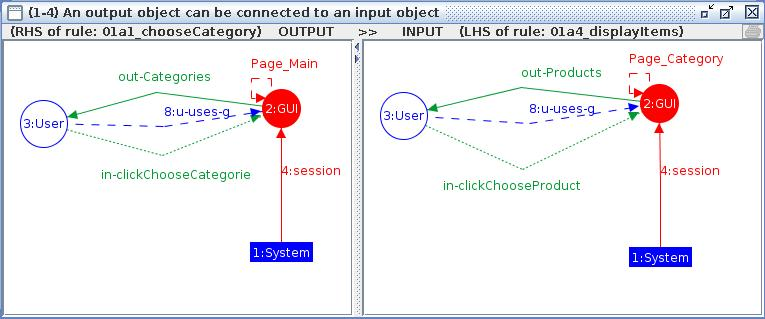
\includegraphics[scale=0.7]{images/generating-tests/grammar/inout}}
  \caption{Input-Output relation building}\label{fig:tests:inout}
\end{figure}

\end{example}

\section{Processing the input grammar}

  Having $GG$ the graph grammar model of the system, $F$ a collection of rules and $IO$ an \emph{input-output relation}, we proceed to the construction of an occurrence graph grammar for $GG$ accomplished by means of an amalgamation of $F$ over its input-output relation $IO$. This amalgamation is later used in the construction of a doubly-typed graph grammar, which we then check to verify if it satisfies the conditions to be an occurrence grammar. The construction steps are specified in Definition~\ref{def:ogg-construction}.

\begin{definition}[Deterministic Occurrence Graph Grammar Construction]\label{def:ogg-construction} Let \graphGrammar{} be a graph grammar, $F$ a functionality collection and $IO$ its corresponding input-output relation:

\begin{enumerate}
  \item\label{enum:construction-colimit} calculate the amalgamation (colimit) $Occ$ of the rules in $F$ with respect to $IO$ as presented in the diagram below, where all squares commute.

\diagram{
  & & & & IO_6\ar[dddrrrr]\ar[dddllll] & & & & \\
    & IO_3\ar[ddl]\ar[ddrrrr] & & & & & & IO_4\ar[ddr]\ar[ddllll] &\\
    & & IO_1\ar[d]\ar[dr] & & IO_5\ar[drr]\ar[dll] & & I O_2\ar[d]\ar[dl] & &\\
    L_1\ar[dddrrrr] & K_1\ar[l]\ar[r] & R_1\ar[dddrr] & L_2\ar[dddr] & K_2\ar[l]\ar[r] & R_2\ar[dddl] & L_3\ar[dddll] & K_3\ar[l]\ar[r] & R_3\ar[dddllll]\\
    & & & & & & & &\\
    & & & & & & & &\\
    & & & & Occ & & & &
}\hfill\break

\hide{
\diagram{
  & & & & IO_6\ar[dddrrrr]\ar[dddllll] & & & & &\ldots\\
    & IO_3\ar[ddl]\ar[ddrrrr] & & & & & & IO_4\ar[ddr]\ar[ddllll] & & \ldots\\
    & & IO_1\ar[d]\ar[dr] & & IO_5\ar[drr]\ar[dll] & & IO_2\ar[d]\ar[dl] & & &\ldots\\
    L_1\ar[dddrrrr] & K_1\ar[l]\ar[r] & R_1\ar[dddrr] & L_2\ar[dddr] & K_2\ar[l]\ar[r] & R_2\ar[dddl] & L_3\ar[dddll] & K_3\ar[l]\ar[r] & R_3\ar[dddllll] & \ldots\ar[dddlllll]\\
    & & & & & & & & &\\
    & & & & & & & & &\\
    & & & & Occ & & & & &
}\hfill\break}

\item retype the rules in $F_\alpha$ over $Occ_\alpha$. In other words, use each morphism found from each $L_i, K_i, R_i$ to $Occ_\alpha$ as their respective new typing morphism. This step generates a set $F'_\alpha$ of doubly-typed graph rules, since $Occ_\alpha$ is itself a $TG$ typed graph.

\item calculate the causal relation $\leq_{c}$ of the doubly-typed graph rules in $F'_\alpha$.

\item\label{enum:construction-graphs} generate the initial and final graphs $I_\alpha$ and $J_\alpha$ by respectively deleting from $Occ_\alpha$ all elements ever created and deleted by the rules in $F'_\alpha$.

\item\label{enum:construction-occurrence} calculate the produce-forbid and delete-forbid relations.

\begin{enumerate}
\item\label{enum:construction-analysis} use the concrete conflicts and dependencies to extend the causal relation in order to obtain the occurrence relation $\leq_o$.

\item\label{enum:construction-restriction} use the abstract conflicts and dependencies to generate the set $R_\alpha$ of restrictions over the ordering of rules applicability.
\end{enumerate}

\item\label{enum:construction-ordering} find one or more total orderings of rules in $F'_\alpha$ which respects both the occurrence relation and the occurrence restrictions.
\end{enumerate}

%  The (Deterministic) Occurrence Graph Grammar representing execution of the functionality $i$ is given by $OGG_i = (Occ_i, I_i,F_i)$, iff $OGG_i$ respects the conditions imposed by Definition~\ref{def:ogg} 
\end{definition}

If all the steps in such a construction can be successfully executed, specially steps~\ref{enum:construction-graphs} and~\ref{enum:construction-ordering}, we have that $OGG_\alpha = (Occ_\alpha, I_\alpha, F'_\alpha)$ is not only a doubly-typed graph grammar, but also a deterministic occurrence graph grammar. This means it is possible to successfully perform all functionalities in the original collection $F_\alpha$. Our approach creates test cases and oracles from $OGG_\alpha$ whether it is in
fact an occurrence graph grammar or not. In the first case, we have tests for success and failure execution paths, whereas in the second we have tests only for the failure ones. Notwithstanding, we regard the failure tests as important because they pinpoint uses of the underlying system where the system itself is supposed to fail, therefore they can not or should not be performed. In the following, we dive into details of each construction step.

\newadd{The first step of the construction, the amalgamation of the rules in $F_\alpha$ w.r.t. $IO_\alpha$, is responsible to ``glue'' the graphs of all rules in one typed graph $Occ_\alpha$, while identifying the items that are meant to be the same throughout the grammar execution. This can be regarded as a mapping which turns generic elements such as \textit{a waiter} and a \textit{a client} into concrete elements such as the waiter named \textit{John} and the client named \textit{Ann}.
Therefore, at the end of this step, $Occ_\alpha$ contains all concrete elements ever to be created, preserved or deleted by any of the rules in the functionality collection $F_\alpha$.}

\newadd{The retyping step is responsible for generating ``new'' graph rules which, rather than being generic descriptions of functionalities, represent executions of those functionalities over a given context. Therefore, a rule which describes the process where a waiter services a client becomes a concrete action where the waiter \textit{John} services the client \textit{Ann}.}
%The set $F'_\alpha$ of doubly-typed graph rules from the colimit calculated in the previous step.
\newadd{For each original graph rule $\mbox{$p^{T} = \left(L^{T} \leftarrow K^{T} \rightarrow R^{T}\right)$} \in F_\alpha$, we generate a new action \mbox{$q^{Occ_\alpha} = \left(L^{Occ_\alpha} \leftarrow K^{Occ_\alpha} \rightarrow R^{Occ_\alpha}\right)$}, where the typing morphisms are those from the original rules to the colimit graph. Since $Occ_\alpha$ is the type graph of the
new rules and, at the same time, a typed graph over $T$, the actions are new doubly-typed rules over $Occ_\alpha^T$.}

\newadd{Once the set $F'_\alpha$ of actions was created, we proceed to the calculating the causal relation, as described in Definition~\ref{def:causal-relation}. This relation is the very first indicative of whether it is possible to construct an occurrence graph grammar for the given collection of rules. Remember that this relation must be a total order, otherwise the functionality is not executable. Specifically, the causal relation gives us hints over the order in which the actions must be
performed to accomplish the functionality aims, for example: \textit{Ann} must be on a
table before she orders a \textit{salad}, \textit{John} can not create a new reservation for, let us say \textit{Alex}, if he has not logged in the system, etc.}

\newadd{The next step consists of using the causal relation and the graph $Occ_\alpha$ in order to generate the initial and final graphs of our target grammar. These graphs correspond to the necessary input and expected output of performing $F_\alpha$. In order to create the graphs, we delete from $Occ_\alpha$ the elements that are created (resp. deleted) by the rules in $F'_\alpha$ according to the causal relation. For example: \textit{Ann} is a person who can never be created by any functionality of our system, no matter how
advanced, as a consequence she must be present in any initial states of the actions performed with her. On
the other hand, her \textit{salad} will only be created after a series of other events were triggered, for instance \textit{Ann} must have entered the restaurant. Thus, her \textit{salad} can not exist at an initial state.}

\newadd{After simply deleting those elements from $Occ_\alpha$, the result may be that either $I_\alpha$ or $J_\alpha$ are not valid graphs, in the case that any source or target node of an edge is deleted, but not the edge itself. This means that, for the execution of $F_\alpha$ to be performed, it would need to begin on or lead to an inconsistent state, therefore no sequencing of action in $F_\alpha$ can be performed in a real execution. However, if they are indeed valid graphs, we just have
found the input and output data for our test case.}

\newadd{Notice that, if the steps listed so far (\ref{enum:construction-colimit} to~\ref{enum:construction-graphs}) were able to be successfully performed, we have a grammar \mbox{$OGG_\alpha = \left(Occ_\alpha, I_\alpha, F'_\alpha\right)$} that is not only doubly-typed, but also strongly safe. Therefore it is a candidate to be an occurrence grammar.}

\newadd{In step~\ref{enum:construction-occurrence}, we proceed towards creating the occurrence relation and occurrence relation restrictions. In~\ref{enum:construction-analysis}, we calculate all produce-forbid conflicts and delete-forbid dependencies between the rules in $F'_\alpha$ by using the categorial algorithms presented in~\ref{def:classic-dependency} and~\ref{def:classic-conflict}. So far, we do not know whether these conflicts and dependencies will be exercised during the execution of our underlying grammar. For example:
a client can not be accommodated at a table reserved for another client. \textit{John} can however accommodate \textit{Ann} at a table specifically reserved for her or at any table not reserved at all. Given the information collected so far we can deduce if this condition exists in this given execution and/or under which conditions it exists. Hence, we use the information acquired in previous steps to classify those conflicts and dependencies as concrete, abstract or non-existent as specified in
Definitions~\ref{def:delete-forbid-strong} and~\ref{def:produce-forbid-strong}.}

\newadd{The occurrence relation $\leq_o$ is then calculated from the causal relation together
with the concrete conflicts and dependencies. In step~\ref{enum:construction-restriction} we create the set $R_i$ of restrictions as the union of all abstract conflicts and dependencies calculated before.}

\newadd{Finally, we have the strongly safe grammar $OGG_i$ together with its corresponding occurrence relation $\leq_o$ and a set of restrictions $R_i$. Therefore, if $\leq_o$ is a partial order and it is possible to find a total ordering of it that respects all restrictions in $R_i$, it follows that $OGG_i$ is an occurrence graph grammar according to Definition~\ref{def:ogg}.}

\hide{If $Occ_i$ is a \emph{core graph} according to definition~\ref{def:core-graph}, we can create a doubly-typed graph grammar $OGG_i$ that is also a strongly-safe grammar and therefore a candidate to be an occurrence graph grammar. Otherwise, it means that there is more than one rule that deletes or creates the same element, therefore it is not possible to apply all rules of this collection and we can build an $OGG_i$ that is a  deterministic occurrence graph grammar.}

\begin{example}[Occurrence Graph Grammar Construction Example]
\end{example}

\important{maybe one more example were the construction fails?}

\begin{example}[Amalgamation example]\label{ex:amalgamation} Figure~\ref{fig:tests:colimit} shows the object resultant from the amalgamation of the rules presented in Figure~\ref{fig:tests:grammar}.

\begin{figure}[!ht]
  \centering
  \fbox{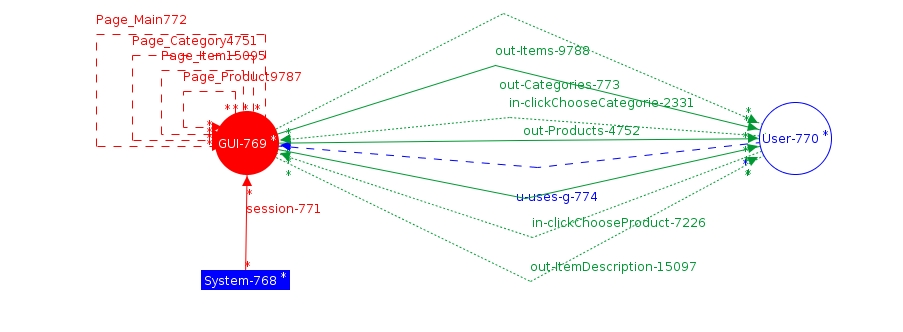
\includegraphics[scale=0.4]{images/generating-tests/colimit}}
  \caption{Amalgamation (colimit) of rules according to the IO relation.}\label{fig:tests:colimit}
\end{figure}
\end{example}

\begin{example}[Initial and Final Graphs Example] Figure~\ref{fig:tests:graphs} shows the initial and final states for the main flow of \emph{browse catalogue}.

\begin{figure}[!ht]
  \centering
  \begin{subfigure}[t]{.5\textwidth}
    \centerline{\fbox{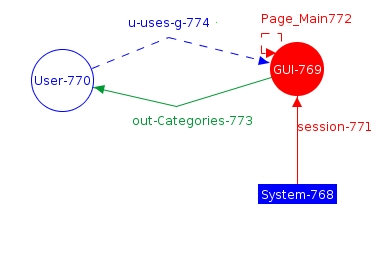
\includegraphics[scale=0.5]{images/generating-tests/grammar/initial}}}
    \caption{Initial graph}
  \end{subfigure}%
  \begin{subfigure}[t]{.5\textwidth}
    \centerline{\fbox{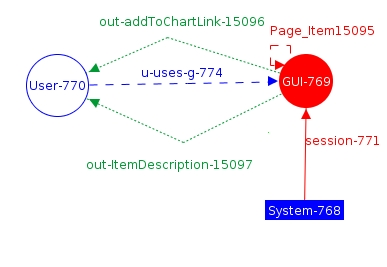
\includegraphics[scale=0.5]{images/generating-tests/grammar/final}}}
    \caption{Final graph}
  \end{subfigure}
  \caption{Instance graphs}\label{fig:tests:graphs}
\end{figure}
\end{example}

\subsection{Implementation} \newadd{The construction of the occurrence graph grammars to generate test cases was implemented in the Verigraph System.}

\begin{figure}[!ht]
\caption{Colimit Implementation}
\begin{minted}[linenos=true, breaklines,fontsize=\small]{haskell}

calculateRulesColimit :: RuleSequence morph -> [NamedRuleWithMatches morph]
calculateRulesColimit (_,rs,os) =
  let
    fs = ksCoproduct rs
    gs = allCoproduct rs 
    -- separates morphism families
    (g1s, g2s, g3s) = groupMorphisms (split gs)
    h1 = induceSpanMorphism fs (zipWith <&> g1s (getLefts rs))
    h2 = induceSpanMorphism fs g2s
    h3 = induceSpanMorphism fs (zipWith <&> g3s (getRights rs))
    coEq = calculateNCoequalizer [h1,h2,h3]
    hm = map (coEq <&> ) gs
    
    -- colimit (based on coequalizers) with object flows
    leftIOs  = map getLeftMorphism os
    rightIOs = map getRightMorphism os
    objCop = objectFlowCoproduct os
    leftFamily = induceSpanMorphism objCop leftIOs
    rightFamily = induceSpanMorphism objCop rightIOs
    coreGraphMorphism = calculateCoequalizer leftFamily rightFamily
    hs2 = split $ map (coreGraphMorphism <&>) hm
  in if null os then zip rs hs1 else zip rs hs2

\end{minted}
\label{fig:tests-colimit}
\end{figure}

\subsection{Analysing results}

Once the previous verifications were successful, we can build the occurrence relation (and any other relation discussed on chapter~\ref{ch:process}) to verify if $OGG_i$ can really be an occurrence graph grammar. If no abstract dependencies or conflicts are found, then the concrete relations are sufficient to do this verification, thus we simply need to check if there is a total ordering compatible with the relations.

\begin{example}[Occurence Relation] Figure~\ref{fig:tests:relation} shows the relation between the rules of this occurrence graph grammar.
\end{example}

If the set $R$ of \emph{occurrence relation restrictions} is not empty, we also need to check if there is a total ordering of the occurrence relation that respects these restrictions.

As this seems to be a hard problem, in the complexity sense, we left this last implementation as a future work. However, we still use the restrictions to generate a set of tests regarding the consistency of the system states.

In our case studies, no such situation was found. We believe that it happens because we used grammars extracted from real use cases, where usually there are (possibly many) sequential connections between the actions, which forces the rules to be connected via the \emph{occurrence relation} and avoids abstract restrictions.

The output of Verigraph for test case generation is shown on Figures~\ref{fig:tests:checklist} and~\ref{fig:tests:relation}. On the first figure, Verigraph performs the basic verifications to check whether the generated output is, in fact, an occurrence grammar.

\begin{figure}[!ht]
\caption{Tool command line output}
\begin{minted}[linenos=true, breaklines,fontsize=\small]{shell}
Testing Serialization:
[OK] Unique creations and deletions
[OK] Initial graph is valid
[OK] Final graph is valid
[OK] Concrete occurrence relation is a total order
[OK] Concrete elements relation is a total order
[OK] There are no abstract restrictions
Analysis written in tmp/output_analysis
Test cases written in tmp/output_test_cases
Saved in tmp/output.ggx
\end{minted}
  \label{fig:tests:checklist}
\end{figure}

\begin{figure}[!ht]
\caption{Output for browse catalogue main flow}
\begin{minted}[linenos=true, breaklines,fontsize=\small]{ruby}
Rules involved: {
["01a1_chooseCategory", "01a2_displayProducts", "01a3_chooseProduct", "01a4_displayItems", "01a5_02b5_chooseItem", "01a6_02b6_displayChosenItem"]
}

Concrete Rules Relation: {
[("01a1_chooseCategory" < "01a2_displayProducts"), ("01a1_chooseCategory" < "01a3_chooseProduct"), ("01a1_chooseCategory" < "01a4_displayItems"), ("01a1_chooseCategory" < "01a5_02b5_chooseItem"), ("01a1_chooseCategory" < "01a6_02b6_displayChosenItem"),...]
}

Elements involved: {
[Node 768,Node 769,Node 770,Edge 771,Edge 772,Edge 773,Edge 774,Edge 2331,Edge 4751,Edge 4752,Edge 7226,Edge 9787,Edge 9788,Edge 15095,Edge 15096,Edge 15097]
}

Elements Relation: {
[(Edge 772 < Edge 4751),(Edge 772 < Edge 4752),(Edge 772 < Edge 7226),(Edge 772 < Edge 9787),(Edge 772 < Edge 9788),(Edge 772 < Edge 15095),(Edge 772 < Edge 15096),(Edge 772 < Edge 15097),(Edge 773 < Edge 4751),(Edge 773 < Edge 4752),(Edge 773 < Edge 7226) ...]
}

Rules Ordering: {
["01a1_chooseCategory","01a2_displayProducts","01a3_chooseProduct", "01a4_displayItems","01a5_02b5_chooseItem", "01a6_02b6_displayChosenItem"]
}

Element Ordering: {
[Node 768,Node 769,Node 770,Edge 771,Edge 772,Edge 773,Edge 774,Edge 2331,Edge 4751,Edge 4752,Edge 7226,Edge 9787,Edge 9788,Edge 15095,Edge 15096,Edge 15097]
}

Set of Abstract Restrictions: {
[]
}
\end{minted}
  \label{fig:tests:relation}
\end{figure}
The analysis file contains the results for calculation of conflicts and dependencies among rules and among elements. The test cases file contains the information relevant to test designer.
The \code{.ggx} presents the occurrence graph grammar constructed, together with its initial and final graphs.

The test oracles are represented by the concrete rules relation and the set of abstract restrictions: any path that complains to the format imposed by them is considered valid and must always succeed. On the other hand, paths that break at least one of such restrictions are considered invalid, and their tests must always capture them as failures.

The tests are represented by the rules and element ordering and also by the initial and final graphs. The ordering of rules is one of (possibly) many valid orders in which the rules can be applied.

The ordering of elements represent an ordering in which the state of the system may be constructed. While the initial and final graphs translate the valid formats for the input and output of each test.

More specific usability details can be found on the Verigraph tutorial, which can be found at \url{https://github.com/Verites/verigraph-tutorial/releases}.

